\usepackage[utf8]{inputenc}
\usepackage{slovak}
\usepackage{tikz}
\usepackage{fancybox}
\usepackage{import}
\usepackage{forloop}
\usepackage{color,soul}
\usepackage{ifthen}
\makeatletter
\newcommand\SoulColor{%
  \let\set@color\beamerorig@set@color
  \let\reset@color\beamerorig@reset@color}
\newcommand\hlif[2]{%
  \ifthenelse{#1}{\SoulColor\hl{#2}}{#2}
}
\makeatother
\usepackage[english]{babel}
\uselanguage{English}
\languagepath{English}
\usetikzlibrary{arrows,positioning}
\usetheme{Warsaw}
\bibliographystyle{apalike}
\title{Sequential P Systems with Active Membranes Working on Sets}
\author{{\bf Michal Kováč}, Damas Gruska}
\institute{Faculty of Mathematics, Physics and Informatics, Comenius University, Bratislava, Slovakia}
\date{30.9.2015}
\begin{document}

\begin{frame}[t]
\titlepage
\end{frame}
\note{}

\section*{Outline}
\begin{frame}
\tableofcontents
\end{frame}
\note{}

\section{Overview of formal models} % (fold)
\label{sec:overview_of_formal_models}

  \subsection{P systems} % (fold)
  \label{sub:p_systems}

    \begin{frame}[t]\frametitle{Membrane structure}
      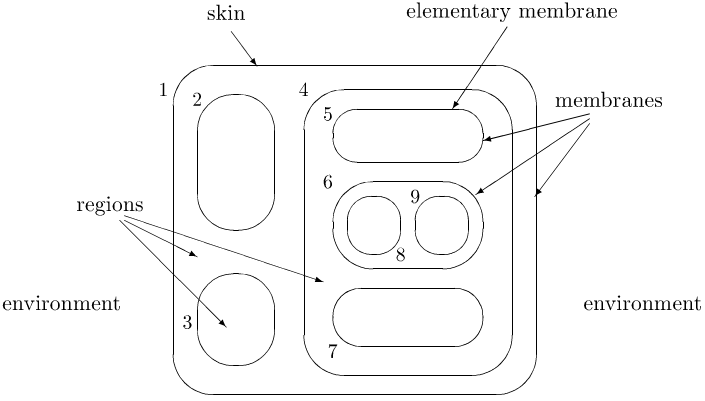
\includegraphics[width=0.7\textwidth]{membrane_structure.png}
      \hfill
      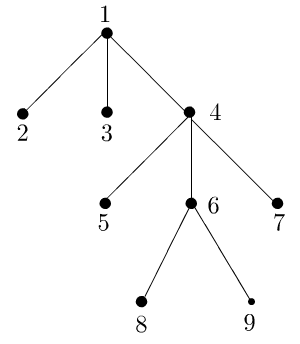
\includegraphics[width=0.3\textwidth]{membrane_tree.png}
      \pause
      \begin{itemize}
        \item Multisets
        \pause
        \item Rewriting rules
        \pause
        \item Passive vs. Active
      \end{itemize}

    \end{frame}
    \note{With active membranes we have a problem when creating a membrane which already exists. We can ignore this fact and let multiple membranes with same label exist beside each other. Then we need to define what is to be done when sending an object to child membrane with a given label. Either the object is copied to each child membrane or one is nondeterministically chosen. A more viable option is to dis }

    \begin{frame}[t]\frametitle{Computation}
      \begin{itemize}
        \item Maximal parallel vs. sequential
        \pause
        \item Language
        \begin{itemize}
          \item Generating mode: language of sequences of objects sent out from the skin membrane
          \item Accepting mode: accept the given configuration if the system can halt
        \end{itemize}
      \end{itemize}

    \end{frame}
    \note{}

  % subsection p_systems (end)

  \subsection{Using sets instead of multisets} % (fold)
  \label{sub:using_sets_instead_of_multisets}
    
    \begin{frame}[t]\frametitle{Using sets instead of multisets}
      \begin{itemize}
        \item How realistic is the counting?
        \item Effectiveness of verification techniques
      \end{itemize}
      
    \end{frame}
    \note{}

    \begin{frame}[t]\frametitle{Set membane systems}
      \begin{itemize}
        \item Alhazov \cite{Alhazov05WithoutMultiplicities}: multiplicities of objects are ignored
        \pause
        \begin{itemize}
          \item maximal parallel $\Rightarrow$ deterministic
          \pause
          \item equivalent to finite state machines
          \pause
          \item with active membranes universal
        \end{itemize}
        \pause
        \item Kleijn, Koutny \cite{Kleijn11SetMembrane}: ``min-enabled'' computational step = sequential
        \pause
        \begin{itemize}
          \item equivalent to finite state machines
        \end{itemize}        
        \pause
        \item Properties:
        \begin{itemize}
          \item No conflict (objects can participate as reactants in as many rules as they want).
          \item If an object is used as a reactant for at least one rule, it is consumed.
        \end{itemize}
      \end{itemize}
    \end{frame}
    \note{}

  % subsection using_sets_instead_of_multisets (end)

% section overview_of_formal_models (end)

\section{Sequential active set membrane systems} % (fold)
\label{sec:sequential_active_set_membrane_systems}

  \subsection{Original semantics} % (fold)
  \label{sub:original_semantics}

    \begin{frame}[t]\frametitle{Sequential active set membrane systems}
      \begin{itemize}
        \item $\Pi = (\Sigma, C_0, R_0, \ldots R_{m-1})$
        \pause
        \item $C = (T, l, c)$
        \begin{itemize}
          \item $l: V(T) \rightarrow \{0, \ldots, m-1\}$
          \item $c: V(T) \rightarrow 2^\Sigma$
        \end{itemize}
        \pause
        \item Rewriting rules
        \begin{itemize}
          \item $u\rightarrow w$
          \item $u\rightarrow w\delta$
          \item $u\rightarrow [_j v_1]_j v_2$,

          where $u \subseteq \Sigma, |u|\geq 1$, $v_1,v_2\subseteq\Sigma$ and $w\subseteq (\Sigma\times\{\cdot, \uparrow, \downarrow_{j}\})$
        \end{itemize}

      \end{itemize}
    \end{frame}
    \note{}

    \begin{frame}[t]\frametitle{Register machine}
      \begin{itemize}
        \item Registers with non-negative values $r_1, r_2, \ldots$
        \item Labeled instructions $i: op$, where $op$ is:
        \begin{itemize}
          \item $add(j, k)$
          \item $sub(j, k, l)$
          \item $halt$
        \end{itemize}
        \item State = (instruction pointer, values of registers)
        \item Step: modify the register value, move the instruction pointer
      \end{itemize}
    \end{frame}

    \begin{frame}[t]\frametitle{Simulation of a register machine}
      Simulation of a register machine (2 registers, 3 instructions):
      \begin{itemize}
        \item $1: sub(1,2,3)$
        \item $2: add(2,1)$
        \item $3: halt$
      \end{itemize}
    \end{frame}
    \note{}

    \newcounter{i}
    \forloop{i}{1}{\value{i} < 19}{

      \def\hlon(#1)(#2){%
        \hlif{\equal{#1}{\value{i}}}{#2}
      }
      \def\hlonboth(#1)(#2)(#3){%
        \hlif{\equal{#1}{\value{i}} \OR \equal{#2}{\value{i}}}{#3}
      }
      \def\hlonallthree(#1)(#2)(#3)(#4){%
        \hlif{\equal{#1}{\value{i}} \OR \equal{#2}{\value{i}} \OR \equal{#3}{\value{i}}}{#4}
      }

      \begin{frame}[t]\frametitle{Example simulation}
        \begin{columns}
          \begin{column}{0.55\textwidth}
            Skin membrane (6 rules):
            \begin{itemize}
              \item \hlonboth(2)(10)($x_1\rightarrow x_1\downarrow_1$), \hlon(13)($x_2\rightarrow x_2\downarrow_2$)
              \item \hlon(7)($x_2t_2\rightarrow [_2 y_1t_2 ]_2$)
              \item \hlon(18)($x_1t_1\rightarrow x_3$)
              \item \hlonboth(9)(17)($y_1\rightarrow x_1$), \hlonboth(6)(12)($y_2\rightarrow x_2$)
            \end{itemize}
            \vspace{-50pt}
            \begin{figure}
              \hspace{-80pt}
              \def\svgwidth{200pt}
              \makebox[\linewidth]{\import{img/sim1/}{\arabic{i}.pdf_tex}}
            \end{figure}
          \end{column}
          \begin{column}{0.45\textwidth}
            Membrane 1 (4 rules):
            \begin{itemize}
              \item \hlon(3)($x_1\rightarrow x_1\downarrow_1$)
              \item \hlonboth(4)(11)($x_1t_1\rightarrow y_2t_1\delta$)
              \item $y_1\rightarrow y_1\uparrow$, \hlon(5)($y_2\rightarrow y_2\uparrow$)
            \end{itemize}
            \vspace{40pt}
            Membrane 2 (4 rules):
            \begin{itemize}
              \item $x_2\rightarrow x_2\downarrow_2$
              \item \hlon(14)($x_2t_2\rightarrow [_2y_1t_2]_2$)
              \item \hlonallthree(8)(15)(16)($y_1\rightarrow y_1\uparrow$), $y_2\rightarrow y_2\uparrow$
            \end{itemize}
            \vspace{25pt}
          \end{column}
        \end{columns}
      \end{frame}
    }
    \note{This simulation is not very efficient. We need to fire number of rules linear on the value of the register affected. That's why we have also proposed alternative simulation with binary encoding of register value. Then, we can achieve logarithimic time overhead. To fully make use of the hierarchical structure we propose some sort of Catalan encoding, which can make the simulation even more efficient.}

  % subsection original_semantics (end)

  \subsection{Modified membrane creation semantics} % (fold)
  \label{sub:modified_membrane_creation_semantics}

    \begin{frame}[t]\frametitle{Issues with original semantics}
      \begin{itemize}
        \item Two issues:
        \begin{enumerate}
          \item Explicit membrane creation rule
          \pause
          \item Sending an object to a child membrane
        \end{enumerate}
        \pause
        \item Alternatives:
        \begin{enumerate}
          \item Inject-or-create (no explicit membrane creation rule)
          \pause
          \item Wrap-or-create
        \end{enumerate}
      \end{itemize}
    \end{frame}
    \note{}

    % INJECT-OR-CREATE

    \begin{frame}[t]\frametitle{Inject-or-create semantics}
      \begin{columns}
        \begin{column}{0.5\textwidth}
          \vspace{-20pt}
          \only<2>{\hspace{50pt}\makebox[\linewidth]{$a\rightarrow a\downarrow_2$}}
          \vspace{-20pt}
          \begin{figure}
            \def\svgwidth{150pt}
            \makebox[\linewidth]{\import{img/inj/}{1.pdf_tex}}
          \end{figure}
          \vspace{-20pt}
          \only<3>{\hspace{50pt}\makebox[\linewidth]{$a\rightarrow a\downarrow_3$}}
        \end{column}
        \begin{column}{0.5\textwidth}
          \onslide<2>
          \vspace{-30pt}
          \begin{figure}
            \def\svgwidth{150pt}
            \makebox[\linewidth]{\import{img/inj/}{2.pdf_tex}}
          \end{figure}
          \onslide<3>
          \vspace{-30pt}
          \begin{figure}
            \def\svgwidth{150pt}
            \makebox[\linewidth]{\import{img/inj/}{3.pdf_tex}}
          \end{figure}    
        \end{column}
      \end{columns}
    \end{frame}
    \note{}

    % WRAP-OR-CREATE
  
    \newcounter{j}
    \forloop{j}{1}{\value{j} < 9}{

      \def\hlon(#1)(#2){%
        \hlif{\equal{#1}{\value{j}}}{#2}
      }
      \def\hlonboth(#1)(#2)(#3){%
        \hlif{\equal{#1}{\value{j}} \OR \equal{#2}{\value{j}}}{#3}
      }

      \begin{frame}[t]\frametitle{Wrap-or-create semantics}
        \begin{columns}
          \begin{column}{0.55\textwidth}
            \vspace{-20pt}
            \begin{figure}
              \hspace{-80pt}
              \def\svgwidth{200pt}
              \makebox[\linewidth]{\import{img/sim2/}{\arabic{j}.pdf_tex}}
            \end{figure}
          \end{column}
          \begin{column}{0.45\textwidth}
            Skin membrane:          
            \begin{itemize}
              \item \hlon(8)($x_1t_1\rightarrow x_3t_1$)
              \item \hlonboth(2)(5)($x_1s_1\rightarrow x_1\downarrow_1$)
              \item \hlon(7)($x_2s_2\rightarrow [_2s_2]_2s_2x_1$)
              \item \hlon(4)($x_2t_2\rightarrow [_2t_2]_2s_2x_1$)
            \end{itemize}
            \vspace{30pt}
            Membrane 1:
            \begin{itemize}
              \item \hlonboth(3)(6)($x_1\rightarrow x_2\delta$)
            \end{itemize}
          \end{column}
        \end{columns}
      \end{frame}
    }

    \begin{frame}[t]{Comparison of membrane creation semantics}
      \begin{center}
        \begin{tabular}{|c|c|c|l|}
          \hline
          semantics & membranes & time & alphabet \\ \hline
          original & $O(n)$ & $O(n)$ & $2*\# instr.+\# reg.$ \\ \hline
          original & $O(log(n))$ & $O(log(n))$ & $3*\# instr.+ 5$ \\ \hline
          inject-or-create & $O(log(n))$ & $O(log(n))$ & $3*\# instr.+ 5$ \\ \hline
          wrap-or-create & $O(n)$ & $O(1)$ & $\# instr.+2*\# reg.$ \\ \hline
        \end{tabular}
      \end{center}
    \end{frame}

  % subsection modified_membrane_creation_semantics (end)

% section sequential_active_set_membrane_systems (end)

\begin{frame}[plain]
  \bibliography{csp}
\end{frame}

\begin{frame}[plain]
  \begin{center}
    Thanks for your attention!
  \end{center}
\end{frame}

\end{document}
